\section{Capítulo 2 -- Complexidade de Algoritmos}

Dois programas podem resolver o mesmo problema e dar a mesma resposta, mas um terminar em um piscar de olhos e o outro levar horas. A diferença quase nunca está no computador: está no algoritmo. Neste capítulo você vai aprender a medir a eficiência de um algoritmo sem precisar executá-lo, usando a notação Big O. Essa ferramenta vai acompanhar você em todos os capítulos seguintes: para cada estrutura de dados, vamos perguntar quanto custa inserir, buscar e remover.

\subsection{2.1 Por que medir a eficiência?}

Imagine um sistema com o cadastro de 1 milhão de clientes. Para encontrar um cliente pelo CPF, você pode olhar um por um, do primeiro ao último. No pior caso, são 1 milhão de comparações. Se o cadastro estiver ordenado, dá para fazer como numa lista telefônica: abrir no meio, ver se o CPF está antes ou depois e descartar metade a cada passo. Assim, bastam cerca de 20 comparações.

Os dois métodos funcionam, mas um é 50 mil vezes mais rápido que o outro. E a diferença aumenta conforme o cadastro cresce. É por isso que analisamos algoritmos: para escolher, antes de programar, a solução que continua viável quando os dados crescem.

A eficiência pode ser medida em dois recursos:

\begin{itemize}
  \item \textbf{Tempo}: quantas operações o algoritmo faz. É a análise mais comum e o foco deste capítulo.
  \item \textbf{Espaço}: quanta memória extra o algoritmo precisa. Veremos na seção 2.8.
\end{itemize}

\subsection{2.2 Medir o tempo ou analisar o algoritmo?}

A forma mais direta de saber se um programa é rápido é executá-lo e cronometrar. Em C++, a biblioteca \texttt{chrono} faz isso:

\begin{codigo}
\begin{Verbatim}[breaklines=true, breaksymbolleft={}, fontsize=\footnotesize]
#include <chrono>

long long somar(int n) {
    long long soma = 0;
    for (int i = 1; i <= n; i++) {
        soma += i;
    }
    return soma;
}

int main() {
    auto inicio = chrono::steady_clock::now();
    long long resultado = somar(100000000);
    auto fim = chrono::steady_clock::now();

    auto ms = chrono::duration_cast<chrono::milliseconds>(fim - inicio).count();
    cout << "Resultado: " << resultado << endl;
    cout << "Tempo: " << ms << " ms" << endl;
}
\end{Verbatim}
\end{codigo}

Essa \textbf{análise experimental} é útil, mas tem limites. O tempo medido depende do processador, do sistema operacional, do compilador, de outros programas abertos e até dos dados usados no teste. Rodando o mesmo código em outra máquina, o número muda. E, para medir, você precisa ter o algoritmo pronto.

A \textbf{análise de complexidade} olha para o algoritmo em si. Em vez de medir segundos, ela conta \textbf{quantas operações} o algoritmo faz em função do tamanho da entrada. O resultado vale para qualquer máquina e pode ser obtido antes de escrever o código. As duas análises se completam: a de complexidade ajuda a escolher o algoritmo, e a experimental ajusta os detalhes quando o tempo é crítico.

\subsection{2.3 Contando operações}

O primeiro passo da análise é definir o \textbf{tamanho da entrada}, que chamamos de $n$. Ele depende do problema:

\begin{center}
\begin{tabular}{@{}p{0.38\linewidth}p{0.48\linewidth}@{}}
\toprule
\rowcolor{headergray}
\tblheader{Problema} & \tblheader{Tamanho da entrada ($n$)} \\
\midrule
Ordenar ou buscar em um vetor & quantidade de elementos \\
\rowcolor{rowgray} Operações em uma lista ou árvore & quantidade de nós \\
Algoritmos em grafos & número de vértices e de arestas \\
\rowcolor{rowgray} Processar um texto & quantidade de caracteres \\
\bottomrule
\end{tabular}
\end{center}

Depois, contamos as operações que importam. Veja a função que soma os elementos de um vetor:

\begin{codigo}
\begin{Verbatim}[breaklines=true, breaksymbolleft={}, fontsize=\footnotesize]
int somarVetor(int v[], int n) {
    int soma = 0;               // 1 vez
    for (int i = 0; i < n; i++) {
        soma += v[i];           // n vezes
    }
    return soma;                // 1 vez
}
\end{Verbatim}
\end{codigo}

A atribuição inicial e o \texttt{return} acontecem uma vez; a soma dentro do laço acontece $n$ vezes. Contando também as comparações e incrementos do \texttt{for}, chegamos a algo como $t(n) = 3n + 3$ operações. O número exato depende de como se conta, e é aí que entra a ideia mais importante do capítulo: \textbf{o que interessa não é o valor exato, e sim como $t(n)$ cresce quando $n$ cresce}. Se o vetor dobrar de tamanho, o trabalho dobra. Esse comportamento é o que a notação Big O captura.

\subsection{2.4 Melhor caso, pior caso e caso médio}

Para muitos algoritmos, o número de operações depende não só do tamanho, mas também do \textbf{conteúdo} da entrada. A busca sequencial é o exemplo clássico:

\begin{codigo}
\begin{Verbatim}[breaklines=true, breaksymbolleft={}, fontsize=\footnotesize]
// devolve a posição do valor procurado, ou -1 se não encontrar
int buscaSequencial(int v[], int n, int procurado) {
    for (int i = 0; i < n; i++) {
        if (v[i] == procurado) {
            return i;
        }
    }
    return -1;
}
\end{Verbatim}
\end{codigo}

\begin{itemize}
  \item \textbf{Melhor caso}: o valor está na primeira posição. Uma comparação basta, não importa o tamanho do vetor.
  \item \textbf{Pior caso}: o valor está na última posição ou não existe. São $n$ comparações.
  \item \textbf{Caso médio}: supondo que o valor esteja no vetor e que qualquer posição seja igualmente provável, em média percorremos metade do vetor, cerca de $n/2$ comparações.
\end{itemize}

O \textbf{pior caso} é o mais usado, por um motivo prático: ele é uma \textbf{garantia}. Se o pior caso de um algoritmo é aceitável, ele nunca vai decepcionar. O melhor caso costuma ser otimista demais para servir de base a uma decisão, e o caso médio exige saber como os dados se distribuem, o que nem sempre é possível.

\subsection{2.5 A notação Big O}

A notação Big O descreve como o tempo de um algoritmo cresce, deixando de lado os detalhes que não mudam esse crescimento. Dizemos que a busca sequencial é $O(n)$ (lê-se ``ó de ene''): no pior caso, o tempo cresce de forma proporcional ao tamanho da entrada.

\subsubsection{A ideia: ficar com o termo que domina}

Suponha que um algoritmo faça $t(n) = 3n^2 + 5n + 20$ operações. Veja quanto cada parte contribui:

\begin{center}
\begin{tabular}{@{}p{0.16\linewidth}p{0.2\linewidth}p{0.14\linewidth}p{0.08\linewidth}p{0.24\linewidth}@{}}
\toprule
\rowcolor{headergray}
\tblheader{$n$} & \tblheader{$3n^2$} & \tblheader{$5n$} & \tblheader{$20$} & \tblheader{parte de $3n^2$} \\
\midrule
10 & 300 & 50 & 20 & 81\% \\
\rowcolor{rowgray} 100 & 30.000 & 500 & 20 & 98,3\% \\
1.000 & 3.000.000 & 5.000 & 20 & 99,8\% \\
\bottomrule
\end{tabular}
\end{center}

Quando $n$ cresce, o termo $n^2$ domina completamente. As constantes (o 3, o 5, o 20) dependem de detalhes de implementação e da máquina. Por isso, a notação Big O fica só com o termo dominante, sem a constante: esse algoritmo é $O(n^2)$.

\subsubsection{A definição formal}

Uma função $t(n)$ é $O(f(n))$ se existem constantes positivas $c$ e $k$ tais que

\[ t(n) \le c \cdot f(n) \quad \text{para todo } n \ge k. \]

Em palavras: a partir de um certo tamanho de entrada ($k$), o tempo do algoritmo nunca passa de um múltiplo ($c$) de $f(n)$. No exemplo acima, com $c = 4$ e $k = 8$, temos $3n^2 + 5n + 20 \le 4n^2$ para todo $n \ge 8$; logo $t(n)$ é $O(n^2)$.

\begin{destaque}{Regras práticas do Big O}
\begin{itemize}
  \item \textbf{Descarte as constantes}: $O(3n)$ é $O(n)$; $O(n^2/2)$ é $O(n^2)$.
  \item \textbf{Fique com o termo de maior crescimento}: $O(n^2 + n)$ é $O(n^2)$; $O(n + \log n)$ é $O(n)$.
  \item \textbf{Trechos em sequência se somam}: um laço $O(n)$ seguido de outro $O(n^2)$ resulta em $O(n^2)$.
  \item \textbf{Trechos aninhados se multiplicam}: um laço de $n$ voltas dentro de outro de $n$ voltas resulta em $O(n \cdot n) = O(n^2)$.
\end{itemize}
\end{destaque}

\subsection{2.6 As principais classes de complexidade}

Quase todos os algoritmos que você vai encontrar se encaixam em poucas classes:

\begin{center}
\begin{tabular}{@{}p{0.17\linewidth}p{0.2\linewidth}p{0.51\linewidth}@{}}
\toprule
\rowcolor{headergray}
\tblheader{Classe} & \tblheader{Nome} & \tblheader{Exemplo} \\
\midrule
$O(1)$ & constante & acessar \texttt{v[i]}; inserir no início de uma lista encadeada \\
\rowcolor{rowgray} $O(\log n)$ & logarítmica & busca binária em vetor ordenado \\
$O(n)$ & linear & busca sequencial; somar um vetor \\
\rowcolor{rowgray} $O(n \log n)$ & linearítmica & merge sort; heapsort \\
$O(n^2)$ & quadrática & bubble sort; comparar todos os pares \\
\rowcolor{rowgray} $O(n^3)$ & cúbica & multiplicação simples de matrizes \\
$O(2^n)$ & exponencial & testar todos os subconjuntos de um conjunto \\
\bottomrule
\end{tabular}
\end{center}

O gráfico mostra como essas funções crescem. Repare como $O(\log n)$ quase não sai do chão, enquanto $O(2^n)$ dispara logo no início:

\begin{center}
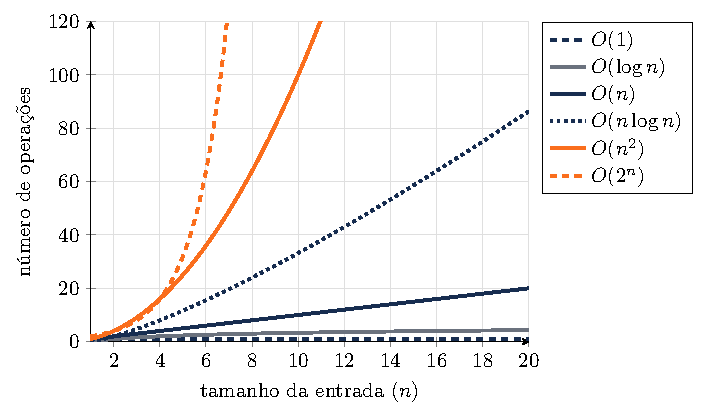
\includegraphics[width=\linewidth,keepaspectratio]{imagens/capitulo-02_crescimento.pdf}
\end{center}

Para sentir a diferença na prática, imagine um computador que faz \textbf{1 milhão de operações por segundo}. Quanto tempo cada classe levaria?

\begin{center}
\begin{tabular}{@{}p{0.2\linewidth}p{0.3\linewidth}p{0.36\linewidth}@{}}
\toprule
\rowcolor{headergray}
\tblheader{Classe} & \tblheader{$n = 1.000$} & \tblheader{$n = 1.000.000$} \\
\midrule
$O(\log n)$ & 10 microssegundos & 20 microssegundos \\
\rowcolor{rowgray} $O(n)$ & 1 milissegundo & 1 segundo \\
$O(n \log n)$ & 10 milissegundos & 20 segundos \\
\rowcolor{rowgray} $O(n^2)$ & 1 segundo & cerca de 11,6 dias \\
$O(2^n)$ & mais que a idade do universo & impossível \\
\bottomrule
\end{tabular}
\end{center}

A tabela explica por que a escolha do algoritmo importa mais que a velocidade do computador. Um processador mil vezes mais rápido transforma os 11,6 dias do $O(n^2)$ em cerca de 17 minutos, mas um algoritmo $O(n \log n)$, na máquina antiga, resolve o mesmo problema em 20 segundos.

\subsection{2.7 Analisando código passo a passo}

Com as regras da seção 2.5, dá para descobrir a complexidade lendo o código. Veja os padrões mais comuns.

\subsubsection{Laço simples: O(n)}

\begin{codigo}
\begin{Verbatim}[breaklines=true, breaksymbolleft={}, fontsize=\footnotesize]
// encontra o maior valor do vetor: percorre cada elemento uma vez
int maiorValor(int v[], int n) {
    int maior = v[0];
    for (int i = 1; i < n; i++) {
        if (v[i] > maior) {
            maior = v[i];
        }
    }
    return maior;
}
\end{Verbatim}
\end{codigo}

\subsubsection{Laços aninhados: O(n²)}

\begin{codigo}
\begin{Verbatim}[breaklines=true, breaksymbolleft={}, fontsize=\footnotesize]
// verifica se o vetor tem algum valor repetido, comparando todos os pares
bool temRepetido(int v[], int n) {
    for (int i = 0; i < n; i++) {
        for (int j = i + 1; j < n; j++) {
            if (v[i] == v[j]) {
                return true;
            }
        }
    }
    return false;
}
\end{Verbatim}
\end{codigo}

O laço interno começa em \texttt{i + 1}, então ele dá $n-1$ voltas, depois $n-2$, e assim por diante. A soma é $n(n-1)/2$ comparações no pior caso. Descartando a constante $1/2$ e o termo menor, a função é $O(n^2)$.

\subsubsection{Laço que divide a entrada: O(log n)}

\begin{codigo}
\begin{Verbatim}[breaklines=true, breaksymbolleft={}, fontsize=\footnotesize]
// quantas vezes n pode ser dividido por 2 até chegar a 1?
int contarDivisoes(int n) {
    int passos = 0;
    while (n > 1) {
        n = n / 2;
        passos++;
    }
    return passos;
}

int main() {
    cout << contarDivisoes(1000) << endl;     // 9
    cout << contarDivisoes(1000000) << endl;  // 19
}
\end{Verbatim}
\end{codigo}

Sempre que um algoritmo \textbf{descarta metade} do problema a cada passo, ele é logarítmico. Multiplicar a entrada por mil acrescenta só uns 10 passos. É o segredo da busca binária (Capítulo 7) e das árvores balanceadas (Capítulo 5).

\subsubsection{Laço que divide dentro de um laço linear: O(n log n)}

\begin{codigo}
\begin{Verbatim}[breaklines=true, breaksymbolleft={}, fontsize=\footnotesize]
int exemploNLogN(int n) {
    int total = 0;
    for (int i = 0; i < n; i++) {           // n vezes
        for (int j = n; j > 1; j = j / 2) { // log n vezes
            total++;
        }
    }
    return total;
}
\end{Verbatim}
\end{codigo}

Esse é o padrão dos bons algoritmos de ordenação, como o merge sort (Capítulo 8): cada um dos $\log n$ níveis de divisão faz um trabalho linear.

\subsubsection{Recursão}

Em Algoritmos I você viu que uma função recursiva chama a si mesma. Para analisá-la, conte quantas chamadas acontecem e quanto trabalho cada uma faz.

\begin{codigo}
\begin{Verbatim}[breaklines=true, breaksymbolleft={}, fontsize=\footnotesize]
// fatorial: n chamadas, cada uma com trabalho constante -> O(n)
long long fatorial(int n) {
    if (n <= 1) return 1;
    return n * fatorial(n - 1);
}

// Fibonacci recursivo: cada chamada gera outras duas -> O(2^n)
long long fibRecursivo(int n) {
    if (n <= 1) return n;
    return fibRecursivo(n - 1) + fibRecursivo(n - 2);
}

// Fibonacci com laço: guarda só os dois últimos valores -> O(n)
long long fibIterativo(int n) {
    long long anterior = 0, atual = 1;
    for (int i = 0; i < n; i++) {
        long long proximo = anterior + atual;
        anterior = atual;
        atual = proximo;
    }
    return anterior;
}

int main() {
    cout << fatorial(10) << endl;      // 3628800
    cout << fibRecursivo(30) << endl;  // 832040, após mais de 1 milhão de chamadas
    cout << fibIterativo(30) << endl;  // 832040, com apenas 30 voltas
}
\end{Verbatim}
\end{codigo}

O Fibonacci recursivo é um ótimo alerta: o código é curto e elegante, mas recalcula os mesmos valores muitas vezes. Para \texttt{fibRecursivo(50)}, seriam bilhões de chamadas. A versão com laço resolve em 50 passos. No Capítulo 9 você vai ver a programação dinâmica, uma técnica que conserta exatamente esse tipo de desperdício.

\begin{destaque}{Comparando com Python}
Em Python, operações que parecem instantâneas podem esconder um laço inteiro. Saber a complexidade delas evita surpresas:

\begin{codigo}
\begin{Verbatim}[breaklines=true, breaksymbolleft={}, fontsize=\footnotesize]
nomes = ["ana", "bia", "caio", "davi"]

print("davi" in nomes)   # O(n): percorre a lista até achar
nomes.append("eva")      # O(1) em média: coloca no fim
nomes.insert(0, "zoe")   # O(n): desloca todos os elementos
nomes.pop()              # O(1): remove do fim
nomes.pop(0)             # O(n): desloca todos os elementos

conjunto = set(nomes)
print("davi" in conjunto)  # O(1) em média: usa tabela hash
\end{Verbatim}
\end{codigo}

Uma linha como \texttt{if x in lista} dentro de um laço transforma um algoritmo que parecia $O(n)$ em $O(n^2)$. Em C++, como você escreve os laços, esse custo fica visível no próprio código.
\end{destaque}

\subsection{2.8 Complexidade de espaço}

A mesma notação mede a \textbf{memória extra} que o algoritmo usa, além da própria entrada.

\begin{itemize}
  \item \texttt{somarVetor} e \texttt{fibIterativo} usam só algumas variáveis, não importa o tamanho de $n$: espaço $O(1)$.
  \item Um algoritmo que cria uma cópia do vetor para trabalhar nela usa espaço $O(n)$.
  \item O \texttt{fatorial} recursivo também usa espaço $O(n)$, mesmo sem criar vetores: cada chamada que ainda não terminou ocupa um espaço na pilha de execução, e há $n$ chamadas abertas ao mesmo tempo.
\end{itemize}

Muitas vezes é possível trocar espaço por tempo: guardar resultados já calculados gasta memória, mas evita refazer contas. Essa troca é a base da programação dinâmica.

\begin{destaque}{Para saber mais: Ômega e Theta}
Além do Big O, existem outras duas notações. A notação $\Omega$ (ômega) indica um \textbf{limite inferior}: o algoritmo faz \textit{pelo menos} aquela quantidade de trabalho. A notação $\Theta$ (theta) indica um \textbf{limite exato}: o crescimento é \textit{exatamente} daquela ordem, nem mais nem menos. Na prática, quando alguém diz ``a busca sequencial é $O(n)$'', costuma querer dizer que o pior caso cresce exatamente como $n$. Nesta apostila, seguindo o uso comum, usaremos o Big O.
\end{destaque}

\subsection{Erros Comuns}

\begin{itemize}
  \item \textbf{Confundir Big O com tempo em segundos.} $O(n)$ não diz quanto tempo o programa leva, e sim como esse tempo cresce. Um algoritmo $O(n)$ pode ser mais lento que um $O(n^2)$ para entradas pequenas.
  \item \textbf{Manter constantes e termos menores.} Escrever $O(2n + 10)$ está tecnicamente certo, mas o correto é simplificar para $O(n)$.
  \item \textbf{Somar quando deveria multiplicar.} Dois laços de $n$ voltas \textit{um depois do outro} dão $O(n)$; \textit{um dentro do outro} dão $O(n^2)$.
  \item \textbf{Esquecer o custo das operações de biblioteca.} Chamar uma função que percorre a estrutura inteira (como \texttt{in} em uma lista do Python) dentro de um laço multiplica a complexidade.
  \item \textbf{Analisar só o melhor caso.} Dizer que a busca sequencial é $O(1)$ porque às vezes o valor está na primeira posição esconde o comportamento real. Use o pior caso como referência.
  \item \textbf{Ignorar o espaço da recursão.} Uma função recursiva com $n$ chamadas abertas ao mesmo tempo usa memória $O(n)$, e com $n$ muito grande pode estourar a pilha de execução.
\end{itemize}
